%%%%%%%%%%%%%%%%%%%%%%%%%%%%%%%%%%%%%%%%%%%%%%%%%%%%%%%%%%%%%%%%%%%%%
% LaTeX Template: Project Titlepage Modified (v 0.1) by rcx
%
% Original Source: http://www.howtotex.com
% Date: February 2014
% 
% This is a title page template which be used for articles & reports.
% 
% This is the modified version of the original Latex template from
% aforementioned website.
% 
%%%%%%%%%%%%%%%%%%%%%%%%%%%%%%%%%%%%%%%%%%%%%%%%%%%%%%%%%%%%%%%%%%%%%%

\documentclass[11pt]{report}
\usepackage[a4paper]{geometry}
\usepackage[myheadings]{fullpage}
\usepackage{fancyhdr}
\usepackage{lastpage}
\usepackage{graphicx, wrapfig, subcaption, setspace, booktabs}
\usepackage[T1]{fontenc}
\usepackage[font=small, labelfont=bf]{caption}
\usepackage{fourier}
\usepackage[protrusion=true, expansion=true]{microtype}
\usepackage[english]{babel}
\usepackage{sectsty}
\usepackage{url, lipsum}
\usepackage{amsmath}

\newcommand{\HRule}[1]{\rule{\linewidth}{#1}}
\onehalfspacing
\setcounter{tocdepth}{5}
\setcounter{secnumdepth}{5}

%-------------------------------------------------------------------------------
% HEADER & FOOTER
%-------------------------------------------------------------------------------
\pagestyle{fancy}
\fancyhf{}
\setlength\headheight{15pt}
\fancyhead[L]{Terrence Ho}
\fancyhead[R]{Experiment 4}
\fancyfoot[R]{Page \thepage\ of \pageref{LastPage}}
%-------------------------------------------------------------------------------
% TITLE PAGE
%-------------------------------------------------------------------------------

\begin{document}

\title{ \normalsize \textsc{Physics 4AL}
        \\ [2.0cm]
        \HRule{0.5pt} \\
        \LARGE \textbf{\uppercase{Experiment 5: Harmonic Oscillator Part I:
        Spring Oscillator}}
        \HRule{2pt} \\ [0.5cm]
        \vspace*{2\baselineskip}}

\date{}

\author{
        Terrence Ho | ID: 804793446 \\ 
        Date of Lab: May 16th, 2017 \\
        Lab Section: Tuesday, 5 P.M.\\
        T.A.: David Bauer\\
        Lab Partners: Robathan Harries}

\maketitle
\tableofcontents
\newpage

%-------------------------------------------------------------------------------
% Section title formatting
\sectionfont{\scshape}
%-------------------------------------------------------------------------------

%-------------------------------------------------------------------------------
% BODY
%-------------------------------------------------------------------------------
\addcontentsline{toc}{section}{Abstract}
\begin{center}
\title{
    \Large \textbf{\uppercase{Investigating Damped and Undamped Oscillations}}
}

T. Ho\footnote{Henry Samueli School of Engineering and Applied Science,
University of California, Los Angeles}
\end{center}

In Newtonian mechanics, a mass suspended on a spring undergoes harmonic motions.
The objective of the experiment was to investigate the motion of damped and
undamped oscillations. Specifically, we wanted to find whether
resonant frequencies in both types of oscillations would be equivalent, as well
as any other observations we could make.  A mass
was hung from a vertical force sensor, and measured both voltage and time, with
magnets providing a damping force. Graphs of voltage vs time were plotted to
find the relationship between these values. Through this, we confirmed the 
experimental resonant frequency closely matched calculated predicted values, which was
0.6799 1/s. We observed the amplitude of an undamped oscillation being near
constant, while an undamped oscillation's amplitude decreased very quickly.
Lastly, values of damping term and Q-factor were also derived from the
experiment. 

\newpage
\begin{figure}[h!]
    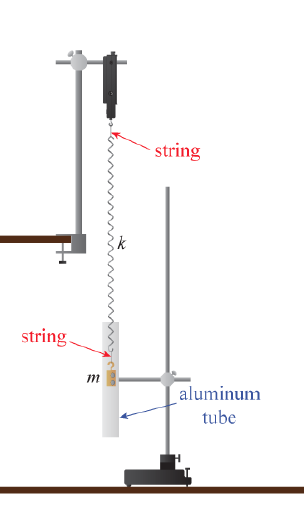
\includegraphics[]{setup.png}
    \captionsetup{labelformat=empty}
    \caption{\textbf{Figure 5.1 Setup for Oscillation Experiment.}  The sensor
    provides the readout of voltage during oscillation motion.  The weight has
    magnets that can provide a damping force if passed through the aluminum
    tube.  Be sure to decouple the spring from the mass and the force sensor to
    produce the most accurate data.  Figure
reproduced (with permission) from Fig. 5.1 by Campbell, W. C. et al.$^1$}
\addcontentsline{toc}{subsection}{Figure 5.1}
\end{figure}

\newpage
\section*{Introduction}
\addcontentsline{toc}{section}{Introduction}
Oscillations are caused by an acting force and a restoring force exerted by a
spring. If an object is oscillating and there is no other force acting on it, it
is in simple harmonic motion and has a constant amplitude and frequency.  This
frequency is also known as the resonant frequency, where it's amplitude will be
greatest.  

In our experiment, we sought to observe both undamped and damped oscillations,
with the ultimate goal of finding the resonant frequency.  By hanging a mass
onto a force sensor and measuring voltage produced by the mass over time,
we can determine the amplitudes, frequencies, and periods by which the mass on
the spring oscillated at.  We can also determine if the resonant frequency is
the same for both undamped and damped oscillations.   


\section*{Methods}
\addcontentsline{toc}{section}{Methods}


The first step of the experiment is to determine the spring constant of the
spring we will hang our masses from.  A series of masses were hung from the
spring and the distance from the mass to the floor was measured and plotted.
The slope of the best fit line gives our spring constant \(k\) (\textbf{Figure
5.2}). 

\textbf{Figure 5.1} shows the layout of our experiment. 
With the force sensor (measuring voltage) attached to the computer, set a high sample
rate for the sensor so voltage data is accurate.  Attach a small string to the
bottom of the hook, then attach the mass to the string (this is done to avoid
uncertainty that occurs when the spring rotates and turns as it stretches and
compresses).  The mass should have magnets on it's side so an aluminnum tube can
be used for the damped oscillation trial and slow the mass.  A small force was
given to the spring mass system and let to oscillate for 40 seconds, during
which voltage and time are recorded.    

Any data recorded should be transferred over to Excel for analysis.  Other data
important to collect would be an offset voltage(to account for the fact the
voltage data may not be centered at zero) and mass of the weight used.  

\section*{Analysis}
\addcontentsline{toc}{section}{Analysis}
We first determined the spring constant of the spring by hanging masses of 0 g, 50 g,
100 g, 150 g, and 200 g, and plotting these masses against the distance
remaining from the ground to the spring when placed onto the spring.  This is
illustrated in \textbf{Figure 5.2}.  The spring constant is determined to be
3.2 $\pm$ 0.2 N/m.

The mass m on the spring we used for our experiment was 175 $\pm$ 0.5 g.  

To predict out resonant frequency, we used the equation \(f_0 =
\frac{1}{2\pi}\sqrt{\frac{k}{m}}\), where \(k\) is the spring constant found on
\textbf{Figure 5.2} and \(m\) is the mass of the weight on spring.  Using the
propagation of uncertainty, \(\frac{\delta f_0}{f_0} =
\sqrt{\bigg(\frac{\delta k}{2k} \bigg)^2 + \bigg(\frac{\delta m}{2m} \bigg)^2}
\), to find the uncertainty for \(f_0\), we find that \(f_{0, predict} = 0.67
\pm 0.2\) Hz. 



\begin{figure}
    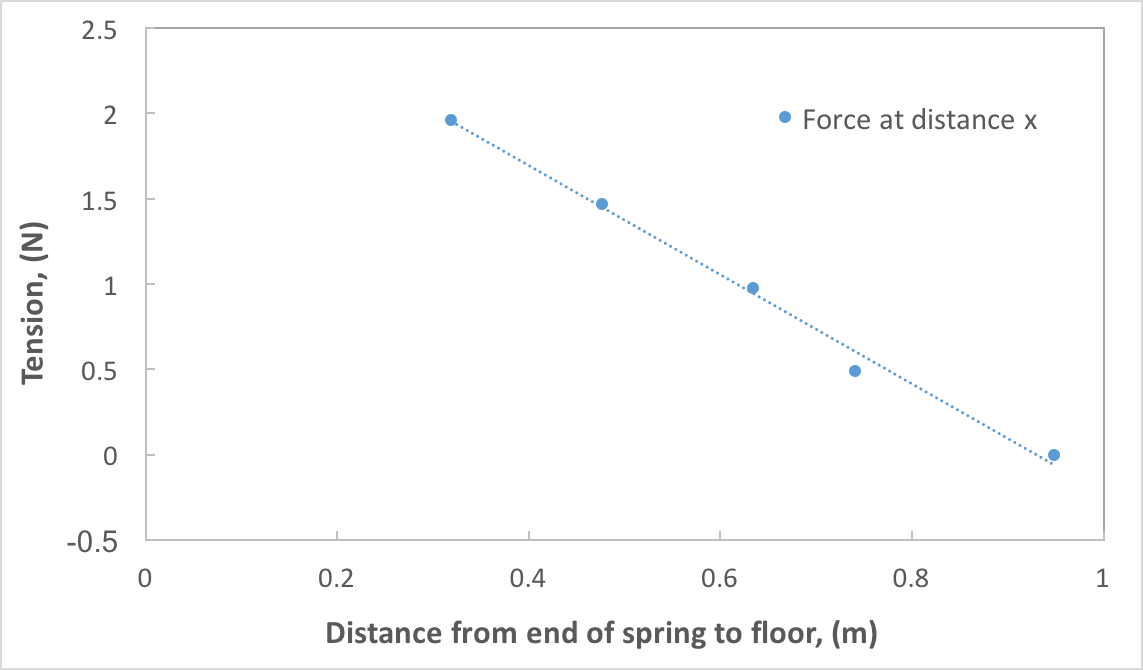
\includegraphics[width=\linewidth]{ForceDistance.png}
    \captionsetup{labelformat=empty}
    \caption{\textbf{Figure 5.2 Measuring Spring Constant of a Spring.}  Masses
    used were 0 g, 50 g, 100 g, 150 g, and 200 g.  The best fit line has the
equation \(F = -3.1945x + 2.9174\) The spring constant was found to be \(3.2 \pm
0.2\).}
\addcontentsline{toc}{subsection}{Figure 5.2}
\end{figure}

\begin{figure}
    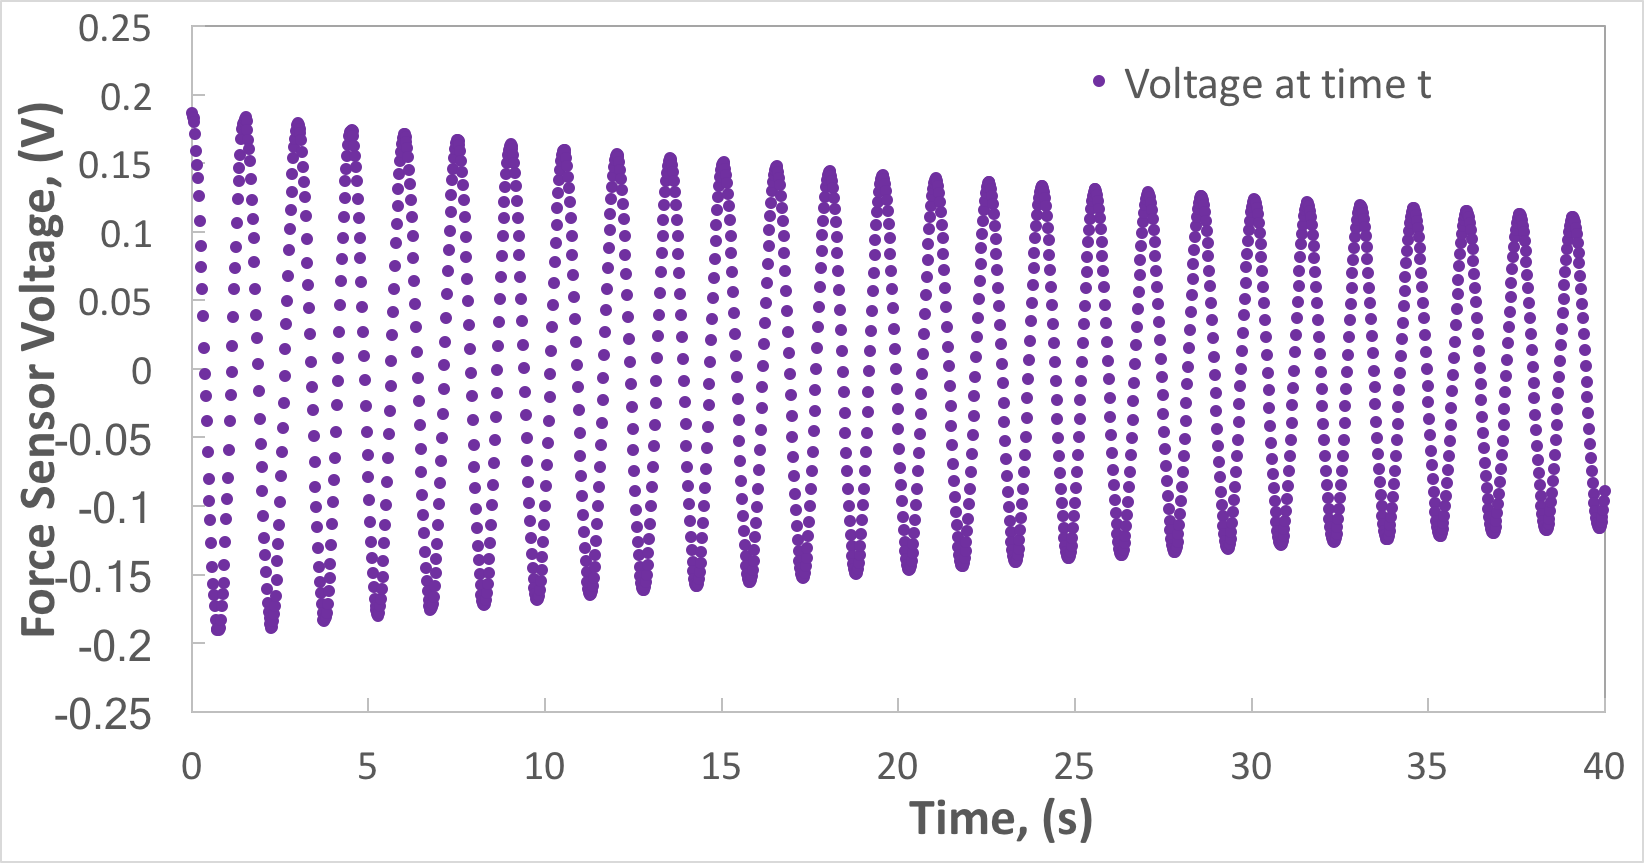
\includegraphics[width=\linewidth]{VoltageTime1.png}
    \captionsetup{labelformat=empty}
    \caption{\textbf{Figure 5.3 Simple Harmonic Motion of Spring.} The x-axis
    shows time of reading and the y-axis shows the voltage measured by the force
sensor at that time. An offset of 0.0327 V was added to each voltage to center
our readings at V = 0.}
\addcontentsline{toc}{subsection}{Figure 5.3}
\end{figure}

In both \textbf{Figure 5.3} and \textbf{Figure 5.4}, we plotted our measured
voltage values at each time. The data is presented with
an offset to the voltage, which accounts for the fact the equilibrium voltage
was not 0 V and to avoid drifting in our data for the damping oscillation in
\textbf{Figure 5.4}.  The offset value is 0.0327 V.

\textbf{Figure 5.3} shows our plotted values of voltage \(V\) at time \(t\) for
the undamped oscillation. We derived our experimental value of $f_{0, undamped}$ by taking the
maxima at several different points, zooming in and finding the maximum value and
time of each peak.  The resonant frequency $f_{0, undamped}$ is then equal to \(\frac{n -
1}{t_n - t_1}\), where \(n\) is the peak number and \(t\) is the time when that
peak occured. We took several trials of this data to find an uncertainty range
(standard deviation of the data divided by the number of trials),
and the resulting frequency was \(f_{0, undamped} = 0.661 \pm 0.002\) Hz.  

Similarly, we plotted the measured voltage values at each time for the damped
oscillation in \textbf{Figure 5.4}. We derived our experimental value of
$f_{damped}$ by taking the
maxima at several different points, zooming in and finding the maximum value and
time of each peak.  The resonant frequency is then equal to \(\frac{n -
1}{t_n - t_1}\), where \(n\) is the peak number and \(t\) is the time when that
peak occured. We took several trials of this data to find an uncertainty range
(standard deviation of the data divided by the number of trials),
and the resulting frequency was \(f_{damped} = 0.660 \pm 0.003\) Hz.  

We can see that in both the damped and undamped oscillations, the resonant
frequencies \(f_0\) calculated from our experiment were within the uncertainty
range of our predicted resonant frequency \(f_{0, predict}\), which was 0.67
$\pm$ 0.02 Hz.  Thus our calculated values are accurate relative to our
predicted value.



\begin{figure}
    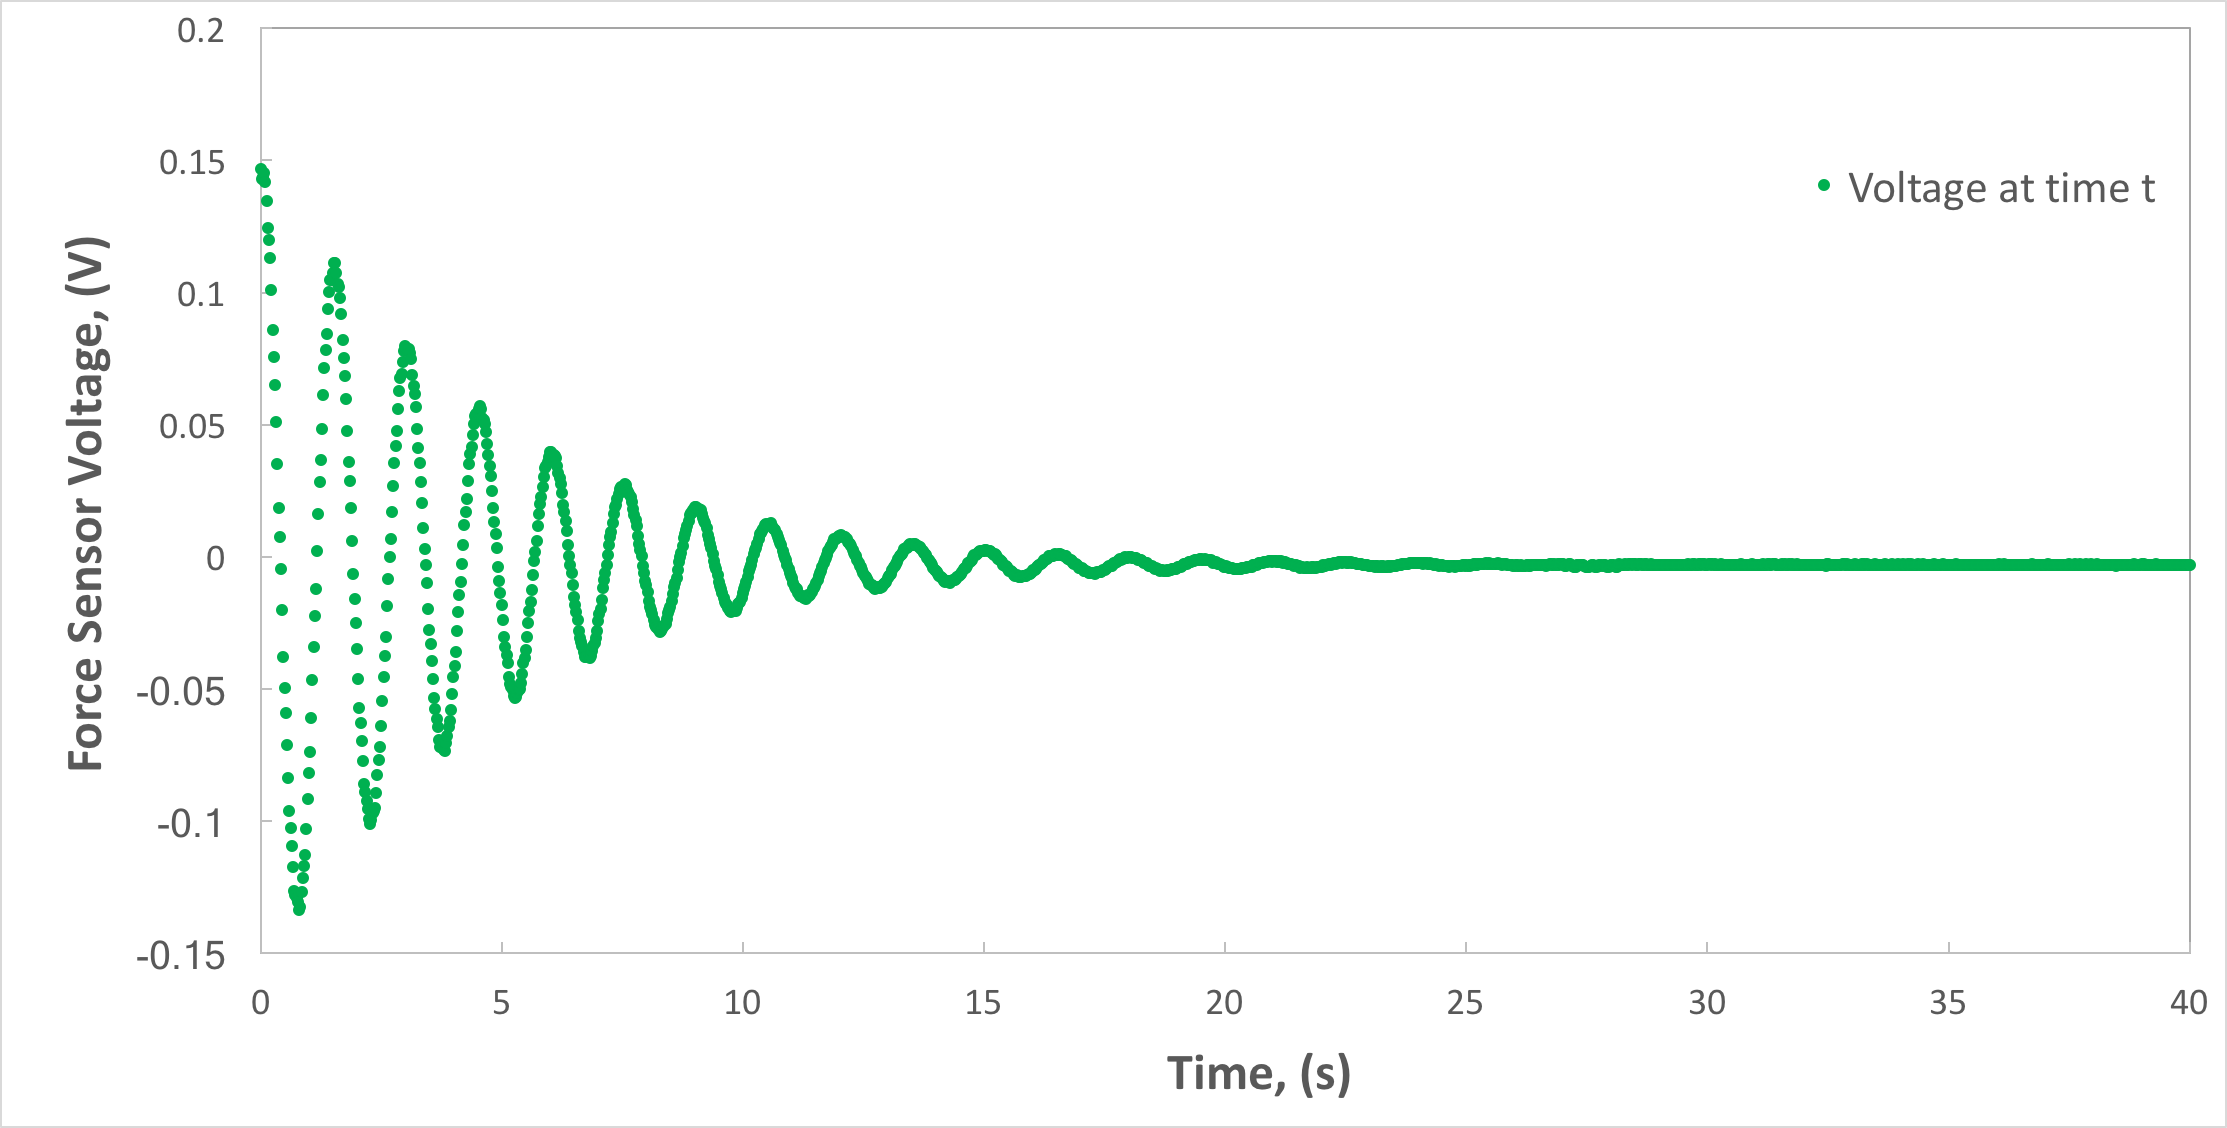
\includegraphics[width=\linewidth]{VoltageTime2.png}
    \captionsetup{labelformat=empty}
    \caption{\textbf{Figure 5.4 Damped Oscillation of a Spring.}  The x-axis
    shows the time of reading and the y-axis shows the voltage measured by the
force sensor at that time.  The offset was 0.0327 V, which was added to each
voltage value to center our readings.}
\addcontentsline{toc}{subsection}{Figure 5.4}
\end{figure}

We can also determine damping time from our graph.  Damping time is 

\begin{figure}
    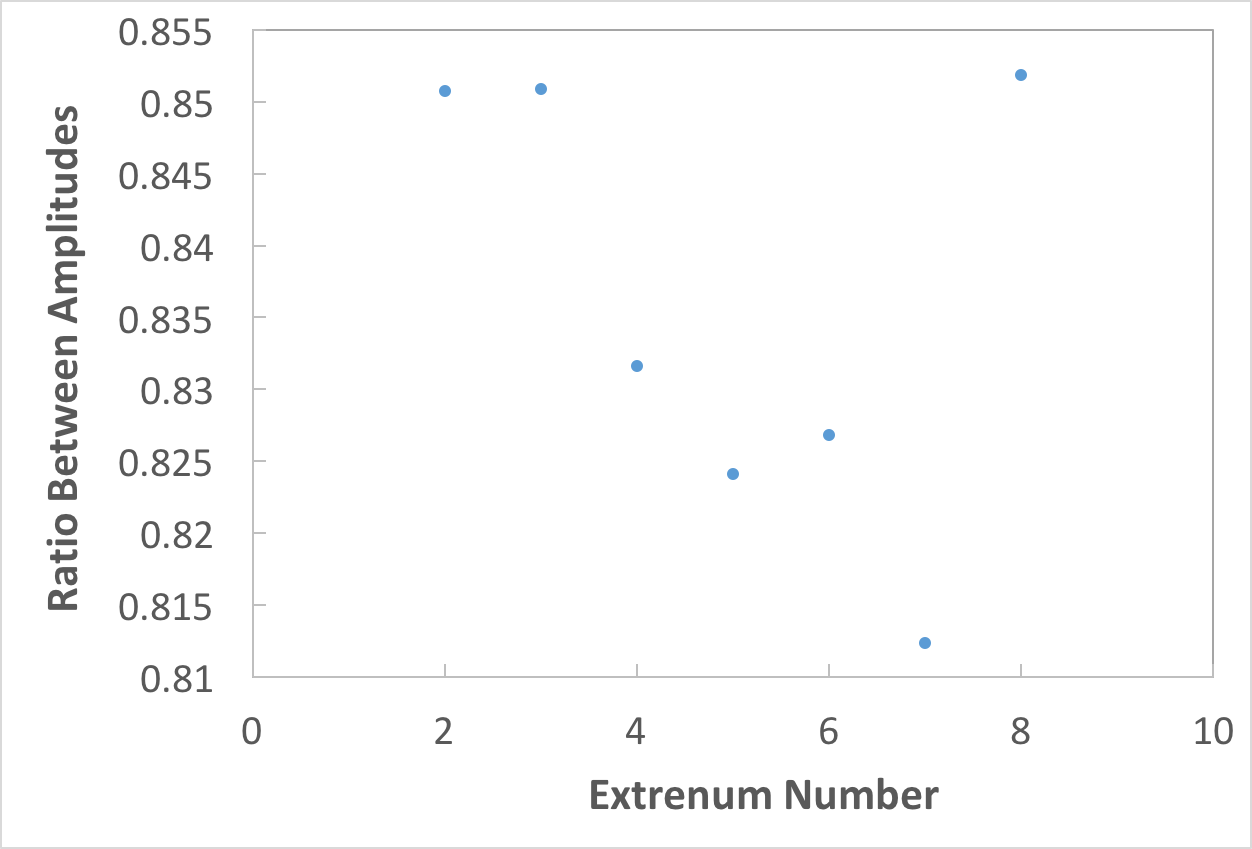
\includegraphics[width=\linewidth]{Extrenum.png}
    \captionsetup{labelformat=empty}
    \caption{\textbf{Figure 5.5 Ratios of Peak Amplitudes}}
    \addcontentsline{toc}{subsection}{Figure 5.5}
\end{figure}


\section*{Conclusion}
\addcontentsline{toc}{section}{Conclusion}
We performed our experiment to study simple harmonic motion and damped
oscillations.  

\newpage
\section*{References}
\addcontentsline{toc}{section}{References}
\begin{enumerate}
    \item Campbell, W. C. et al. Physics 4AL: Mechanics Lab Manual (ver. April
        3, 2017). (Univ. California Los Angeles, Los Angeles, California).
\end{enumerate}




\end{document}



%-------------------------------------------------------------------------------
% REFERENCES
%-------------------------------------------------------------------------------
% \newpage
% \section*{References}
% \addcontentsline{toc}{section}{References}

% Anand, U., 2010. The Elusive Free Radicals, \textit{The Clinical Chemist,} [e-journal] Available at:<\url{http://www.clinchem.org/content/56/10/1649.full.pdf}> [Accessed 2 November 2013]
% \newline
% \newline

% Biology Forums, 2012. \textit{Normal glomerulus. Acute glomerulonephritis.} [online] Available at: <\url{http://biology-forums.com/index.php?action=gallery;sa=view;id=9284}> [Accessed 23 October 2013].
% \newline
% \newline

% Budisavljevic, M., Hodge, L., Barber, K., Fulmer, J., Durazo-Arvizu, R., Self, S., Kuhlmann, M., Raymond, J. and Greene, E., 2003. Oxidative stress in the pathogenesis of experimental mesangial proliferative glomerulonephritis, \textit{American Journal of Physiology - Renal Physiology,} 285(6), pp. 1138-1148.
% \newline
% \newline

% Chien, C., Lee, P., Chen, C., Ma, M., Lai, M. and Hsu, S., 2001. De Novo Demonstration and Co-localization of Free-Radical Production and Apoptosis Formation in Rat Kidney Subjected to Ischemia/Reperfusion, \textit{Journal of the American Society of Nephrology,} 12(5), pp. 973-982.
% \newline
% \newline

% Couser, W., 1993. Pathogenesis of glomerulonephritis, \textit{Kidney International Supplements,} 42, pp. 19-26.
% \newline
% \newline

% De Gasparo, M., 2002. Angiotensin II and nitric oxide interaction, \textit{Heart Failure Reviews,} [e-journal] Available at:<\url{http://www.ncbi.nlm.nih.gov/pubmed/12379820}> [Accessed 26 October 2013]
% \newline
% \newline

% Edinburgh Renal Education Pages, 2012. \textit{Glomerulonephritis} [online] Available at: <\url{http://www.edrep.org/pages/textbook/glomerulonephritis.php}> [Accessed 25 October 2013].
% \newline
% \newline

% Forbes, J., Coughlan, M. and Cooper, M., 2008. Oxidative Stress as a Major Culprit in Kidney Disease in Diabetes, \textit{Diabetes,} 57(6), pp. 1446-1454.
% \newline
% \newline

% Geeky Medics, 2010. \textit{Glomerulonephritis} [online] Available at: <\url{http://geekymedics.com/2010/10/27/glomerulonephritis/}> [Accessed 25 October 2013].
% \newline
% \newline

% Gryglewski, R., Palmer, R., Moncada, S., 1986. Superoxide anion is involved in the break­down of endothelium derived relaxing factor, \textit{Nature,} 320, pp. 454-456.
% \newline
% \newline

% Halliwell, B., 2001. Free Radicals and other reactive species in Disease, \textit{Encyclopedia of Life Sciences,} [e-journal] Available at:<\url{http://web.sls.hw.ac.uk/teaching/level4/bcm1_2/reading/oxidative_stress/files/Oxidative_stress.pdf}> [Accessed 19 October 2013]
% \newline
% \newline

% Huang, H., Patel, P. and Salahudeen, A., 2001. Lazaroid compounds prevent early but not late stages of oxidant-induced cell injury: potential explanation for the lack of efficacy of lazaroids in clinical trials, \textit{Pharmacological Research,} 41(1), pp. 55-61.
% \newline
% \newline

% Klinger, J., Abman, S. and Gladwin, M., 2013. Nitric Oxide Deficiency and Endothelial Dysfunction in Pulmonary Arterial Hypertension, \textit{American Journal of Respiratory and Critical Care Medicine,} 188(6), pp. 639-646.
% \newline
% \newline

% Lindemann, I., Boettcher, J., Oertel, K., Pasternack, R., Heine, A. and Klebe, G. 2012. Inhibitors of Transglutaminase 2: A therapeutic option in celiac disease, \textit{To be Published,} [e-journal + PDB structure] Available at:<\url{http://www.ebi.ac.uk/pdbe-srv/view/entry/3s3s/summary}> [Accessed 24 October 2013]
% \newline
% \newline

% Mayo Clinic, 2011. \textit{Glomerulonephritis} [online] Available at: <\url{http://www.mayoclinic.com/health/glomerulonephritis/DS00503/}> [Accessed 20 October 2013].
% \newline
% \newline

% McCord, J., Roy, R. and Schaffer, S., 1985. Free radicals and myocardial ischemia. The role of xanthine oxidase, \textit{Advances in myocardiology,} [e-journal] Available at:<\url{http://www.ncbi.nlm.nih.gov/pubmed/2982206}> [Accessed 24 October 2013]
% \newline
% \newline

% National Health Service, 2012. \textit{Causes of glomerulonephritis} [online] Available at: <\url{http://www.nhs.uk/Conditions/Glomerulonephritis/Pages/Causes.aspx}> [Accessed 20 October 2013].
% \newline
% \newline

% Niaudet, P., 2013. \textit{Overview of the pathogenesis and causes of glomerulonephritis in children.} [online] Available at: <\url{http://www.uptodate.com/contents/overview-of- \ the-pathogenesis-and-causes-of-glomerulonephritis-in-children}> [Accessed 21 October 2013].
% \newline
% \newline

% Ronco, P., 2013. \textit{Mechanisms of glomerular crescent formation.} [online] Available at: <\url{http://www.uptodate.com/contents/mechanisms-of-glomerular-crescent-formation}> [Accessed 21 October 2013].
% \newline
% \newline

% Rutchik, J., 2013. \textit{Toxic Neuropathy Clinical Presentation.} [online] Available at: <\url{http://emedicine.medscape.com/article/1175276-clinical#a0216}> [Accessed 26 October 2013].
% \newline
% \newline

% R\&D Systems, 2013. \textit{Technical Information. Ischemia/Reperfusion Injury.} [online] Available at: <\url{http://www.rndsystems.com/cb_detail_objectname_SP96_Ischemia.aspx}> [Accessed 28 October 2013].
% \newline
% \newline

% Salahudeen, A., 1999. Free Radicals in Kidney Disease and Transplantation, \textit{Saudi Journal of Kidney Diseases and Transplantation,} 10(2), pp. 137-143.
% \newline
% \newline

% Sarma, A., Mallick, A. and Ghosh, A., 2010. Free Radicals and Their Role in Different Clinical Conditions: An Overview, \textit{International Journal of Pharma Sciences and Research,} 1(3), pp. 182-192.
% \newline
% \newline

% Shah, S., Baliga, R., Rajapurkar, M. and Fonseca, V., 2007. Oxidants in Chronic Kidney Disease, \textit{Journal of the American Society of Nephrology,} 18(1), pp. 16-28.
% \newline
% \newline

% The University of Utah, Unknown. \textit{Glomerulonephritis} [online] Available at: <\url{http://library.med.utah.edu/WebPath/RENAHTML/RENALIDX.html#8}> [Accessed 25 October 2013].
% \newline
% \newline

% Wang, C. and Salahudeen, A., 1994. Cyclosporine nephrotoxicity: attenuation by an antioxidant -inhibitor of lipid peroxidation in-vitro and in-vivo, \textit{Transplantation,} 58, pp. 940-946.
% \newline
% \newline

% Wang, C. and Salahudeen, A., 1995. Lipid peroxidation accompanies cyclosporine nephrotoxicity: effects of vitamin E, \textit{Kidney International,} 47, pp. 927-934.
% \newline
% \newline

% Weiss, S., 1989. Tissue Destruction by Neutrophils, \textit{New England Journal of Medicine,} 320, pp. 365-376.
% \newline
% \newline



%-------------------------------------------------------------------------------
% SNIPPETS
%-------------------------------------------------------------------------------

%\begin{figure}[!ht]
%    \centering
%    \includegraphics[width=0.8\textwidth]{file_name}
%    \caption{}
%    \centering
%    \label{label:file_name}
%\end{figure}

%\begin{figure}[!ht]
%    \centering
%    \includegraphics[width=0.8\textwidth]{graph}
%    \caption{Blood pressure ranges and associated level of hypertension (American Heart Association, 2013).}
%    \centering
%    \label{label:graph}
%\end{figure}

%\begin{wrapfigure}{r}{0.30\textwidth}
%    \vspace{-40pt}
%    \begin{center}
%        \includegraphics[width=0.29\textwidth]{file_name}
%    \end{center}
%    \vspace{-20pt}
%    \caption{}
%    \label{label:file_name}
%\end{wrapfigure}

%\begin{wrapfigure}{r}{0.45\textwidth}
%    \begin{center}
%        \includegraphics[width=0.29\textwidth]{manometer}
%    \end{center}
%    \caption{Aneroid sphygmomanometer with stethoscope (Medicalexpo, 2012).}
%    \label{label:manometer}
%\end{wrapfigure}

%\begin{table}[!ht]\footnotesize
%    \centering
%    \begin{tabular}{cccccc}
%    \toprule
%    \multicolumn{2}{c} {Pearson's correlation test} & \multicolumn{4}{c} {Independent t-test} \\
%    \midrule    
%    \multicolumn{2}{c} {Gender} & \multicolumn{2}{c} {Activity level} & \multicolumn{2}{c} {Gender} \\
%    \midrule
%    Males & Females & 1st level & 6th level & Males & Females \\
%    \midrule
%    \multicolumn{2}{c} {BMI vs. SP} & \multicolumn{2}{c} {Systolic pressure} & \multicolumn{2}{c} {Systolic Pressure} \\
%    \multicolumn{2}{c} {BMI vs. DP} & \multicolumn{2}{c} {Diastolic pressure} & \multicolumn{2}{c} {Diastolic pressure} \\
%    \multicolumn{2}{c} {BMI vs. MAP} & \multicolumn{2}{c} {MAP} & \multicolumn{2}{c} {MAP} \\
%    \multicolumn{2}{c} {W:H ratio vs. SP} & \multicolumn{2}{c} {BMI} & \multicolumn{2}{c} {BMI} \\
%    \multicolumn{2}{c} {W:H ratio vs. DP} & \multicolumn{2}{c} {W:H ratio} & \multicolumn{2}{c} {W:H ratio} \\
%    \multicolumn{2}{c} {W:H ratio vs. MAP} & \multicolumn{2}{c} {\% Body fat} & \multicolumn{2}{c} {\% Body fat} \\
%    \multicolumn{2}{c} {} & \multicolumn{2}{c} {Height} & \multicolumn{2}{c} {Height} \\
%    \multicolumn{2}{c} {} & \multicolumn{2}{c} {Weight} & \multicolumn{2}{c} {Weight} \\
%    \multicolumn{2}{c} {} & \multicolumn{2}{c} {Heart rate} & \multicolumn{2}{c} {Heart rate} \\
%    \bottomrule
%    \end{tabular}
%    \caption{Parameters that were analysed and related statistical test performed for current study. BMI - body mass index; SP - systolic pressure; DP - diastolic pressure; MAP - mean arterial pressure; W:H ratio - waist to hip ratio.}
%    \label{label:tests}
%\end{table}
